\section{Challenges}

\subsection{Relational Modeling}

A large portion of time leading to the completion of the project was attributed to understanding how subjects should be linked. This process was judged to be difficult since some domain requirements can be ambiguous. To resolve this issue, an experiment was conducted using the three main subjects of the domain: agents (search algorithms), puzzles (graphs), and nodes (board states).
\\
\\

(i) Agents use a puzzles and nodes. 
\\

(ii) Puzzles use agents and nodes.
\\

(iii) Each agent uses puzzles and nodes.
\\

(iv) Each puzzle uses agents and nodes.
\\
\\

When the models were compared on the same data set, it was observed that the average run-time for models (i) to (iv) was 2 minutes, 66 ms, 102 ms, and 18 ms respectively.  Moreover, results of the experiment led to two important findings that helped us classify the domain requirements of the project.\\

The first finding resolves the concern of whether or not to use agent or puzzle as the primary subject of the system. For example, should (i/iii) be chosen over (i/iv)? If agent was the primary subject, then each agent must have a reference to a puzzle, and each agent would rely on the puzzle to provide it with a new state for every step of a traversal. The issue with this is that each agent had similar implementations for traversing the puzzle. This affected the overall performance of our system because there were redundancies for the traversal behaviour. To resolve this issue, we took away the responsibility of traversing nodes from the agent class and assigned it to the puzzle class. As a result of this change, the agent's responsibility was now limited to computing heuristic values. Overall, this finding suggests against using (i) and (iii) as a schema for modelling the system.\\

The first finding also suggests that agents should not have direct access to the node class. Yet, having access to this object is important for the system to function properly since it stores the values of each heuristic. A first approach to this problem was to include an accesssor method in the puzzle class. However, this increased the time complexity for state searching by a linear factor, and also contradicts the schema proposed in (ii) and (iv). Therefore, the puzzle needs to reference the agent.\\

\begin{figure}[H]
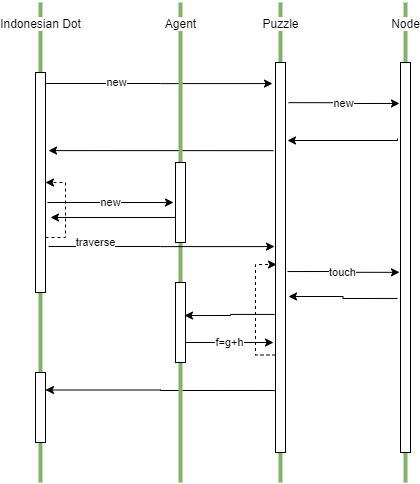
\includegraphics[width=0.75\linewidth]{assets/functional.png}
\caption{Sequence Diagram of Indonesian Dot Solver} \label{fig1}
\end{figure}

This leads to the second finding: A puzzle and an agent cannot have a many-to-many relational type because agent no longer has a reference to a puzzle. Moreover, many nodes are used by one puzzle. Therefore, the combination of both the agent and the node identifies the puzzle that it belongs to. This makes sense since each node points to it's predecessor, with the root node uniquely linked to the puzzle it belongs to (assuming there are no duplicate lines in the test file). Therefore, the second finding suggests that the logical architecture should be modelled after statement (iv).\\

Overall, by performing this experimentation and discovering why the logical architecture performed well under different scenarios, we were able to create a classification plan for classifying each domain requirement into one that belongs to agents, puzzles, or nodes. This experimentation also helped us maximize the performance of the overall system.

\begin{figure}[H]
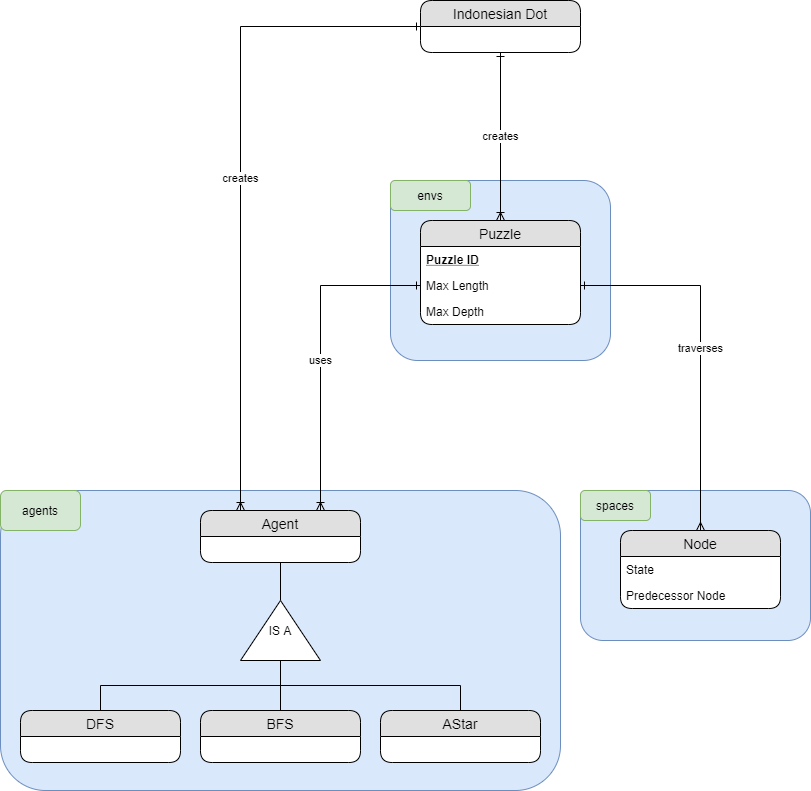
\includegraphics[width=0.75\linewidth]{assets/schema.png}
\caption{Entity Relationship Diagram of Indonesian Dot Solver} \label{fig2}
\end{figure}

\subsection{Touch Redundancy}

Every state of the Indonesian Dot puzzle has actions equivalent to the size of the board. For example, if the board size 25 (or 5x5), then there are 25 actions to choose from. Whenever a traversal was made, it used to be that the puzzle object would touch every action on a node and if it was visited, then it would ignore the action. Yet, checking is an expensive operation especially when the board size increases in size. The touch redundancy issue refers to the issue of having to check for $\sum_{i=0}^{n} {{n!}\over{(n-i)!}} $ actions in the worst case, where $n$ is the total size of the board. This is depicted in the following Figure: 

\begin{figure}[H]
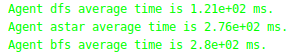
\includegraphics[width=0.75\linewidth]{assets/touch_redundancy.png}
\caption{Average Run Time of DFS, BFS, and A* on 7 Puzzles with Touch Redundancy Issue} \label{fig3}
\end{figure}

To resolve this issue, we discovered that the order of actions leading to the goal state did not matter. More formally, the solution path (in actions) can be any combination of the solution set. This also implies that the system would check for $\sum_{i=0}^{n} {n\choose{i}} = 2^n$ actions in the worst case. This discovery greatly helped reduce the run time of the system:


\begin{figure}[H]
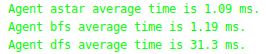
\includegraphics[width=0.75\linewidth]{assets/touch_redundancy_2.png}
\caption{Average Run Time of DFS, BFS, and A* on 7 Puzzles without Touch Redundancy Issue} \label{fig4}
\end{figure}